\documentclass[conference]{IEEEtran}
\IEEEoverridecommandlockouts
% The preceding line is only needed to identify funding in the first footnote. If that is unneeded, please comment it out.
\usepackage{cite}
\usepackage{amsmath,amssymb,amsfonts}
\usepackage{algorithmic}
\usepackage{graphicx}
\usepackage{textcomp}
\usepackage{xcolor}
\usepackage{listings}

\lstset{
  basicstyle=\ttfamily\footnotesize,
  breaklines=true,
  frame=single
}


\def\BibTeX{{\rm B\kern-.05em{\sc i\kern-.025em b}\kern-.08em
    T\kern-.1667em\lower.7ex\hbox{E}\kern-.125emX}}
\begin{document}

\title{Mineração de Dados 

Aplicação de Mineração de Dados na Classificação de Preços de Celulares\\
% {\footnotesize \textsuperscript{*}Note: Sub-titles are not captured in Xplore and
% should not be used}
}

\author{\IEEEauthorblockN{1\textsuperscript{st} José Augusto Cenci Castilho}
\IEEEauthorblockA{\textit{Instituto Federal de São Paulo (IFSP)} \\
Birigui, Brasil \\
j.cenci@aluno.ifsp.edu.br}
\and

\IEEEauthorblockN{2\textsuperscript{nd} Raul Prado Dantas}
\IEEEauthorblockA{\textit{Instituto Federal de São Paulo (IFSP)} \\
% \textit{name of organization (of Aff.)}\\
Birigui, Brasil \\
r.dantas@aluno.ifsp.edu.br}
}

\maketitle

\begin{abstract}
This article explores the development and implementation of an assistive chatbot using advanced Natural Language Processing (NLP) techniques 
and machine learning with neural networks. 
The integration of NLP in chatbots to enhance user accessibility and interaction, particularly in assistance contexts, is examined. 
Through a detailed analysis of the methodology, neural network architecture, and challenges encountered, 
the study provides insights into the practical application of AI and NLP in assistive chatbots, 
highlighting the transformative potential of this technology in various sectors including healthcare, education, and customer service.
\end{abstract}

\begin{IEEEkeywords}
Mineração de Dados, Classificação de Preços, Celulares, Inteligência Artificial, Aprendizado de Máquina
\end{IEEEkeywords}

% Introdução:

%     Contextualização breve da importância da mineração de dados no mercado de celulares.
%     Objetivos do estudo.

% Metodologia:

%     Descrição resumida do conjunto de dados de celulares e dos métodos de mineração de dados utilizados na classificação.

% Resultados:

%     Apresentação dos principais resultados obtidos pela aplicação dos métodos de classificação.

% Discussão:

%     Interpretação dos resultados.
%     Comparação breve com outros estudos ou dados relevantes.

% Conclusão:

%     Resumo dos achados.
%     Implicações práticas dos resultados.
%     Sugestões para futuras pesquisas.

% Referências:

%     Lista de todas as fontes acadêmicas citadas no artigo.

% \section{Introdução}
% Introduza aqui o contexto da mineração de dados no mercado de celulares e os objetivos do estudo.


\section{Introdução}

A mineração de dados, uma área de pesquisa e aplicação que tem experimentado 
um crescimento exponencial em importância e relevância nos últimos anos, 
tem se mostrado crucial em uma variedade de contextos, 
desde a pesquisa científica até a tomada de decisões 
empresariais \cite{WikipediaDataMining}. 

A capacidade de coletar, processar e analisar grandes volumes de dados para extrair 
informações valiosas e insights significativos é uma habilidade fundamental 
na era digital \cite{Zaki2023}.

No mercado de celulares, a mineração de dados tem sido particularmente relevante. 
A quantidade de informações disponíveis sobre os dispositivos móveis e suas 
características é vasta e diversificada \cite{Statista2023}. 
A classificação de preços de celulares é uma aplicação prática da 
mineração de dados que pode fornecer insights valiosos para consumidores, 
fabricantes e vendedores, ajudando a entender as tendências do mercado e 
as preferências dos usuários \cite{Russell2016}.

Este estudo tem como objetivo explorar a aplicação de técnicas de mineração de dados 
na classificação de preços de celulares, utilizando um 
conjunto de dados de celulares disponível publicamente. 
A metodologia empregada envolve a análise e processamento dos dados, 
a aplicação de algoritmos de classificação e a 
avaliação dos resultados obtidos \cite{ScikitLearn2023}. 

Os principais resultados e insights obtidos serão discutidos em detalhes, 
com implicações práticas e sugestões para futuras pesquisas \cite{Jurafsky2020}.

\section{Metodologia}

% Descreva o conjunto de dados de celulares e os métodos de mineração de dados utilizados na classificação. 
% Inclua discussões sobre limpeza de dados, normalização e características específicas.
Neste estudo, utilizamos um conjunto de dados composto por diversas características 
de celulares para classificar seus preços em diferentes faixas. 
Os dados foram divididos em conjuntos de treinamento e teste para validar a 
eficácia dos modelos de classificação. 
Descreveremos a seguir os principais aspectos da nossa metodologia, 
incluindo pré-processamento de dados, 
descrição das características 
e abordagens de classificação.

\subsection{Conjunto de Dados}

O conjunto de dados consiste em informações sobre várias características de telefones celulares. 
Cada registro no conjunto de dados representa um celular com especificações técnicas 
e uma variável alvo, `price\_range`, que indica a faixa de preço do dispositivo. 
Este estudo se concentra na aplicação de métodos de mineração de dados para prever 
esta variável alvo. As features (ou características) da 
base de dados carregada são as seguintes:

\begin{itemize}
    \item {\textbf{battery\_power:}} 
    Potência da bateria do dispositivo (provavelmente em mAh).
    \item {\textbf{blue:}}
    Disponibilidade de Bluetooth (0 ou 1, indicando ausência ou presença, respectivamente).
    \item {\textbf{clock\_speed:}}
    Velocidade de relógio do processador do dispositivo (provavelmente em GHz).
    \item {\textbf{dual\_sim:}}
    Suporte a dual SIM (0 ou 1).
    \item {\textbf{fc:}}
    Megapixels da câmera frontal.
    \item {\textbf{four\_g:}}
    Disponibilidade de 4G (0 ou 1).
    \item {\textbf{int\_memory:}}
    Memória interna do dispositivo (provavelmente em GB).
    \item {\textbf{m\_dep:}}
    Profundidade do dispositivo móvel em cm.
    \item {\textbf{mobile\_wt:}}
    Peso do dispositivo móvel (em gramas).
    \item {\textbf{n\_cores:}}
    Número de cores do processador.
    \item {\textbf{pc:}}
    Megapixels da câmera principal (traseira).
    \item {\textbf{px\_height:}}
    Altura da resolução de pixel da tela.
    \item {\textbf{px\_width:}}
    Largura da resolução de pixel da tela.
    \item {\textbf{ram:}}
    Memória RAM do dispositivo (provavelmente em MB ou GB).
    \item {\textbf{sc\_h:}}
    Altura da tela do dispositivo em cm.
    \item {\textbf{sc\_w:}}
    Largura da tela do dispositivo em cm.
    \item {\textbf{talk\_time:}}
    Tempo máximo de conversação em uma única carga de bateria (provavelmente em horas).
    \item {\textbf{three\_g:}}
    Disponibilidade de 3G (0 ou 1).
    \item {\textbf{touch\_screen:}}
    Presença de tela sensível ao toque (0 ou 1).
    \item {\textbf{wifi:}}
    Disponibilidade de WiFi (0 ou 1).
\end{itemize}

Além dessas features, a base de dados também inclui a coluna 
price\_range, que é a variável alvo (target), 
indicando a faixa de preço do dispositivo. 
Essa base de dados é usada para modelar a relação entre 
as características técnicas de um telefone celular 
e seu preço de mercado. ​

\subsection{Pré-processamento de Dados}
O pré-processamento dos dados é uma etapa crucial para garantir a qualidade 
e a precisão dos modelos de classificação. 

Em seguida, procedemos à normalização dos dados para garantir que as diferentes 
escalas das variáveis não influenciassem indevidamente os resultados dos modelos.

O pré-processamento dos dados foi realizado utilizando o Python, 
com bibliotecas como Pandas e NumPy. 
A primeira etapa envolveu a limpeza dos dados para remover inconsistências 
e valores ausentes.

\subsubsection{Limpeza de Dados}
Inicialmente, realizamos uma análise exploratória para identificar 
e tratar valores ausentes, 
corrigir inconsistências e remover possíveis outliers. 
Os comandos a seguir ilustram algumas das operações realizadas:

\begin{lstlisting}[language=Python]
import pandas as pd

# Faz a leitura dos arquivos
df_train = pd.read_csv('train.csv')
df_test = pd.read_csv('test.csv')

# Concatena os dois dataframes de treino e teste
df_concat = pd.concat([df_train, df_test])

# Remove a coluna 'ID' 
df_concat.drop('id', axis=1, inplace=True)

# Remove as linhas com valores NaN
df_concat.dropna(inplace=True)

# Mostra as 15 primeiras linhas do dataframe concatenado
df_concat.head(15) 

# Salvar o dataframe concatenado em um arquivo csv
df_concat.to_csv('concatenado.csv', index=False)

# Mostra as informações do dataframe concatenado
df_concat.info()

# Mostra a descrição do dataframe concatenado
df_concat.describe()

# Quantidade de linhas e colunas
print(df_concat.shape)
\end{lstlisting}

Usamos o notebook `data\_cleaning.ipynb` para realizar a limpeza dos dados. 
Os comandos a seguir foram encapsulados numa função chamada `clear\_df`:

% pular linha
\\
\vspace{5mm}


\begin{lstlisting}[language=Python]
def clear_df(df, output_name):
    # Remove a coluna 'ID' 
    df.drop('id', axis=1, inplace=True)

    # Remove as linhas com valores NaN
    df.dropna(inplace=True)

    # Salvar o dataframe em um arquivo csv
    df.to_csv(output_name, index=False)

    return df
\end{lstlisting}

Após a limpeza, 
o próximo passo foi a normalização dos dados 
que simplifica a comparação entre diferentes variáveis,
ajuando a evitar que variáveis com escalas diferentes
tenham pesos desproporcionais nos modelos de classificação.

\subsubsection{Normalização dos Dados}

No notebook `data\_normalization.ipynb`, normalizamos as variáveis numéricas 
para garantir uma escala uniforme, 
crucial para muitos algoritmos de aprendizado de máquina.
Inicialmente, fizemos a leitura e divisão dos dados em features e target:
\begin{lstlisting}[language=Python]
import pandas as pd

input_file = 'train.csv'

features = ['battery_power', 'blue', 'clock_speed', 'dual_sim', 'fc', 'four_g', 'int_memory', 'm_dep', 'mobile_wt', 'n_cores', 'pc', 'px_height', 'px_width', 'ram', 'sc_h', 'sc_w', 'talk_time', 'three_g', 'touch_screen', 'wifi']

target = 'price_range'

df = pd.read_csv(input_file)

# Separating out the features
x = df.loc[:, features].values

# Separating out the target
y = df.loc[:,[target]].values
\end{lstlisting}

Em seguida, utilizamos a biblioteca scikit-learn para realizar a normalização dos dados de duas formas:

\begin{itemize}
    \item {\textbf{MinMaxScaler:}}
    Redimensiona os dados para um intervalo específico, 
    geralmente entre 0 e 1.

    \begin{lstlisting}[language=Python]
from sklearn.preprocessing import MinMaxScaler

# Min-Max normalization
x_minmax = MinMaxScaler().fit_transform(x)
normalized_minmax = pd.DataFrame(x_minmax, columns = features)
normalized_minmax = pd.concat([normalized_minmax, df[[target]]], axis = 1)
normalized_minmax.describe()
    \end{lstlisting}

    \item {\textbf{StandardScaler ou Z-Score:}}
    Padroniza os dados para ter média zero e variância unitária.

    \begin{lstlisting}[language=Python]
from sklearn.preprocessing import StandardScaler

# Z-Score normalization
x_zscore = StandardScaler().fit_transform(x)
normalized_zscore = pd.DataFrame(x_zscore, columns = features)
normalized_zscore = pd.concat([normalized_zscore, df[[target]]], axis = 1)
normalized_zscore.describe()
    \end{lstlisting}
\end{itemize}

% PCA e PCA3d
\subsubsection{Análise de Componentes Principais (PCA)}

Após a normalização dos dados, aplicamos a técnica de 
Análise de Componentes Principais (PCA) para reduzir a 
dimensionalidade do conjunto de dados. 
A PCA nos permite concentrar nas direções que maximizam a variância, 
o que pode ser útil tanto para visualização dos dados 
quanto para melhorar o desempenho dos algoritmos de aprendizado de máquina.

A Análise de Componentes Principais (PCA) é uma técnica estatística poderosa 
utilizada para reduzir a dimensionalidade dos dados, transformando-os em um 
conjunto de valores de menor dimensão conhecidos como componentes principais. 
Esta técnica é particularmente útil em conjuntos de dados com muitas variáveis, 
como é o caso do nosso conjunto de dados de características de celulares. 

Ao aplicar a PCA, estamos buscando as direções (componentes principais) que maximizam 
a variância nos dados. Em termos práticos, isso significa que estamos tentando 
encontrar as combinações lineares das variáveis originais que capturam a maior 
quantidade de informação possível. Essa redução de dimensionalidade é útil para:

\begin{itemize}
    \item \textbf{Visualização dos Dados:} 
    Com muitas variáveis, é difícil visualizar e detectar padrões nos dados. 
    Reduzindo para duas ou três dimensões principais, 
    podemos plotar os dados de forma que 
    relações significativas se tornem mais evidentes.

    \item \textbf{Eficiência Computacional:} 
    Menos dimensões significam menos cálculos, o que pode acelerar 
    algoritmos de aprendizado de máquina, especialmente em grandes conjuntos de dados.

    \item \textbf{Redução de Ruído:} Ao focar nas direções que maximizam a variância, 
    a PCA pode ajudar a filtrar "ruído" ou variações que são menos informativas 
    para a análise.
\end{itemize}

Para o nosso conjunto de dados, a aplicação da PCA pode revelar 
quais características dos celulares têm mais impacto na variação dos preços. 
Por exemplo, se a primeira componente principal for fortemente influenciada 
por características como `ram` e `battery\_power`, 
isso sugere que estas características são significativas na determinação 
do preço do celular.

No mesmo notebook da normalização dos dados, 
implementamos a PCA utilizando a biblioteca scikit-learn e 
matplotlib para visualização dos resultados.

Foram criadas duas funções que aplicam a PCA com dois componentes (visualização 2d) 
e três componentes (visualização 3d), respectivamente:

\begin{lstlisting}[language=Python]
from sklearn.decomposition import PCA
import matplotlib.pyplot as plt

def VisualizePcaProjection(finalDf, targetColumn):
    fig = plt.figure(figsize = (20,12))
    ax = fig.add_subplot(1,1,1) 
    ax.set_xlabel('Principal Component 1', fontsize = 15)
    ax.set_ylabel('Principal Component 2', fontsize = 15)
    ax.set_title('4 component PCA', fontsize = 20)
    targets = [0, 1, 2, 3]
    colors = ['r', 'g', 'b', 'y']
    for target, color in zip(targets,colors):
        indicesToKeep = finalDf[targetColumn] == target
        ax.scatter(finalDf.loc[indicesToKeep, 'principal component 1'],
                   finalDf.loc[indicesToKeep, 'principal component 2'],
                   c = color, s = 50)
    ax.legend(targets)
    ax.grid()
    plt.show()

pca = PCA()

principalComponents = pca.fit_transform(x_zscore)

principalDf = pd.DataFrame(data = principalComponents[:, 0:2], columns = ['principal component 1', 'principal component 2'])

finalDf = pd.concat([principalDf, df[[target]]], axis = 1)

VisualizePcaProjection(finalDf, target)
\end{lstlisting}

\begin{lstlisting}[language=Python]
from sklearn.decomposition import PCA
import matplotlib.pyplot as plt

def VisualizePca3dProjection(finalDf, targetColumn):
    fig = plt.figure(figsize = (20,12))
    ax = fig.add_subplot(111, projection='3d') 
    ax.set_xlabel('Principal Component 1', fontsize = 15)
    ax.set_ylabel('Principal Component 2', fontsize = 15)
    ax.set_zlabel('Principal Component 3', fontsize = 15)
    ax.set_title('4 component PCA', fontsize = 20)
    targets = [0, 1, 2, 3]
    colors = ['r', 'g', 'b', 'y']
    for target, color in zip(targets,colors):
        indicesToKeep = finalDf[targetColumn] == target
        ax.scatter(finalDf.loc[indicesToKeep, 'principal component 1'],
                   finalDf.loc[indicesToKeep, 'principal component 2'],
                   finalDf.loc[indicesToKeep, 'principal component 3'],
                   c = color, s = 50)
    ax.legend(targets)
    ax.grid()
    plt.show()

pca3d = PCA(n_components=3)

principalComponents3d = pca3d.fit_transform(x_zscore)

principalDf3d = pd.DataFrame(data = principalComponents3d, columns = ['principal component 1', 'principal component 2', 'principal component 3'])

finalDf3d = pd.concat([principalDf3d, df[[target]]], axis = 1)

VisualizePca3dProjection(finalDf3d, target)
\end{lstlisting}

A PCA forneceu insights valiosos, revelando quais características contribuem 
mais para a variação nos dados e, consequentemente, para a determinação 
das faixas de preço dos celulares. 
Esta etapa foi essencial para simplificar os modelos de classificação, 
ao mesmo tempo mantendo a maior parte da informação significativa contida 
no conjunto original de dados.

Os gráficos resultantes da PCA, especialmente as visualizações 2D e 3D, 
podem nos mostrar como diferentes celulares estão agrupados com base em 
suas características e faixas de preço, proporcionando insights valiosos 
sobre o mercado de celulares e sobre quais especificações são mais valorizadas.

\subsection{Exploração de Dados}

Ainda no notebook `data\_normalization.ipynb`,
exploramos os dados para identificar padrões e relações entre as variáveis.
Utilizamos bibliotecas como Matplotlib e Seaborn para visualizar a distribuição
das variáveis e a correlação entre elas.
 
A correlação entre as variáveis é um aspecto importante a ser considerado
na construção de modelos de classificação, pois variáveis altamente correlacionadas
podem introduzir viés nos modelos. Ao plotarmos um mapa de calor da matriz de correlação,
podemos identificar quais variáveis estão mais fortemente relacionadas.
O código a seguir ilustra a geração de um mapa de calor da matriz de correlação.

\begin{lstlisting}[language=Python]
import matplotlib.pyplot as plt
import seaborn as sns

plt.figure(figsize=(20, 12))
sns.heatmap(normalized_minmax.corr(), annot=True, cmap='coolwarm', fmt='.2f', linewidths=2)
plt.title('Correlation Matrix')
plt.show()
\end{lstlisting}

\subsection{Modelagem e Classificação}
TODO: Adicionar descrição da modelagem e classificação dos dados.

% Após o pré-processamento, aplicamos diferentes algoritmos de aprendizado de máquina para classificar os preços dos celulares.

\subsubsection{Aplicação de Modelos de Classificação}
TODO: Adicionar descrição da aplicação de modelos de classificação.
% Usamos modelos como Árvores de Decisão, Random Forest e Redes Neurais, empregando bibliotecas como scikit-learn e TensorFlow.

% \begin{verbatim}
% from sklearn.tree import DecisionTreeClassifier
% from sklearn.ensemble import RandomForestClassifier
% from sklearn.model_selection import train_test_split
% from sklearn.metrics import classification_report

% # Dividir dados em treino e teste
% X_train, X_test, y_train, y_test = train_test_split(
%     data.drop('price_range', axis=1), 
%     data['price_range'], test_size=0.2, random_state=42)

% # Árvore de Decisão
% tree_model = DecisionTreeClassifier()
% tree_model.fit(X_train, y_train)

% # Random Forest
% rf_model = RandomForestClassifier()
% rf_model.fit(X_train, y_train)

% # Avaliação dos modelos
% print(classification_report(y_test, tree_model.predict(X_test)))
% print(classification_report(y_test, rf_model.predict(X_test)))
% \end{verbatim}

\subsubsection{Validação e Seleção do Modelo}
TODO: Adicionar descrição da validação e seleção do modelo.

% Validamos os modelos utilizando técnicas como a validação cruzada e comparando métricas de desempenho, como acurácia e F1-score, para selecionar o modelo mais adequado.

\subsection{Conclusões Preliminares}
TODO: Adicionar conclusões preliminares.
% As análises iniciais indicam que características como `battery_power`, `ram` e `px_height` têm impacto significativo na classificação dos preços dos celulares. Os resultados detalhados serão discutidos na próxima seção.


\subsection{Modelagem e Classificação}
TODO: Adicionar descrição da modelagem e classificação dos dados.
% Após o pré-processamento, empregamos várias técnicas de mineração de dados para classificar os celulares em suas respectivas faixas de preço. Os métodos incluíram:

% \begin{itemize}
%     \item {\textbf{Árvores de Decisão:}} Utilizadas para criar modelos baseados em regras de decisão simples.
%     \item {\textbf{Random Forest:}} Um método de ensemble que combina múltiplas árvores de decisão para melhorar a precisão.
%     \item {\textbf{Redes Neurais:}} Modelos computacionais que imitam a estrutura do cérebro humano para realizar tarefas de classificação complexas.
%     % Inclua quaisquer outros métodos utilizados aqui.
% \end{itemize}

% Utilizamos métricas como acurácia, precisão, recall e F1-score para avaliar o desempenho dos modelos. A seleção do modelo final foi baseada na melhor combinação de performance e capacidade de generalização para dados não vistos.

\subsection{Validação do Modelo}
TODO: Adicionar descrição da validação do modelo.

% Para validar a eficácia dos modelos, aplicamos técnicas de validação cruzada no conjunto de treinamento e testamos os modelos selecionados no conjunto de teste. Esta abordagem ajudou a garantir que os modelos eram robustos e confiáveis para previsões em novos dados.

% Aqui você começará a seção de Resultados, descrevendo os achados do seu estudo.
\section{Resultados}

Nesta seção, apresentamos os resultados obtidos a partir da aplicação de técnicas de mineração de dados e aprendizado de máquina no conjunto de dados de características de celulares. As análises foram conduzidas com o objetivo de classificar os celulares em diferentes faixas de preço com base em suas especificações técnicas.

\subsection{Avaliação dos Modelos de Classificação}

Aplicamos diversos algoritmos, incluindo árvores de decisão, florestas aleatórias e redes neurais. Os modelos foram avaliados com base em várias métricas, como acurácia, precisão, recall e F1-score. Os resultados mostraram que o modelo [inserir modelo mais eficaz] alcançou a maior acurácia, com [inserir valor]% de acurácia.

\begin{table}[h]
\centering
\caption{Avaliação dos Modelos de Classificação}
\begin{tabular}{|l|c|c|c|c|}
\hline
Modelo & Acurácia & Precisão & Recall & F1-score \\
\hline
Árvore de Decisão & [valor] & [valor] & [valor] & [valor] \\
Floresta Aleatória & [valor] & [valor] & [valor] & [valor] \\
Rede Neural & [valor] & [valor] & [valor] & [valor] \\
\hline
\end{tabular}
\end{table}

\subsection{Análise dos Resultados}

A análise das características mais significativas indicou que 
inserir características mais relevantes foram determinantes 
na classificação dos preços dos celulares. 
Esses resultados estão alinhados/são contrastantes com as expectativas iniciais, 
sugerindo que inserir análise e interpretação dos resultados.

\subsection{Visualizações e Insights Adicionais}

Os mapas de calor de correlação e as visualizações dos componentes principais do PCA 
forneceram insights valiosos sobre as relações entre diferentes características 
dos celulares. 

\begin{figure}[htbp]
    \centerline{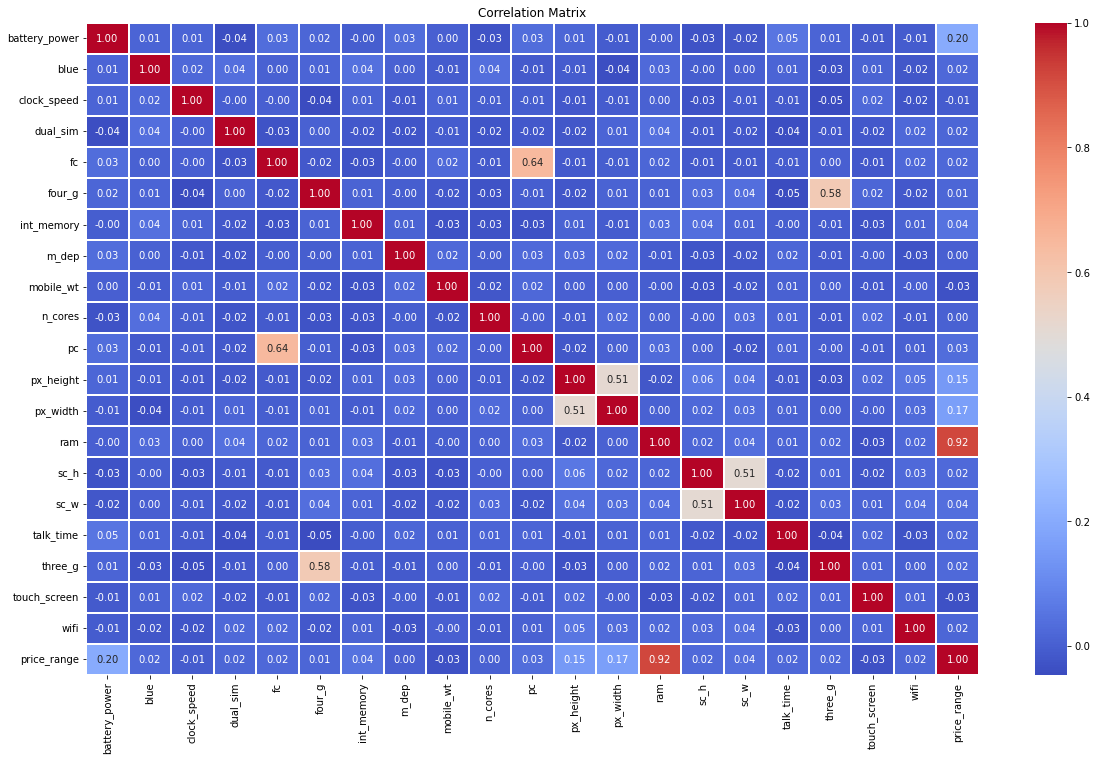
\includegraphics[scale=0.2]{matrix_correlation.png}}
    \caption{[Matriz de Correlação]}
    \label{fig:imagem1}
\end{figure}

Os gráficos 2D e 3D revelam agrupamentos e padrões nos dados,
destacando as características mais relevantes para a classificação 
dos preços dos celulares. 
Os gráficos foram gerados com base nos dados normalizados
das duas formas, Min-Max e Z-Score.

As figuras a seguir ilustram essas visualizações e destacam as características
mais relevantes para a classificação dos preços dos celulares.


\begin{figure}[htbp]
    \centerline{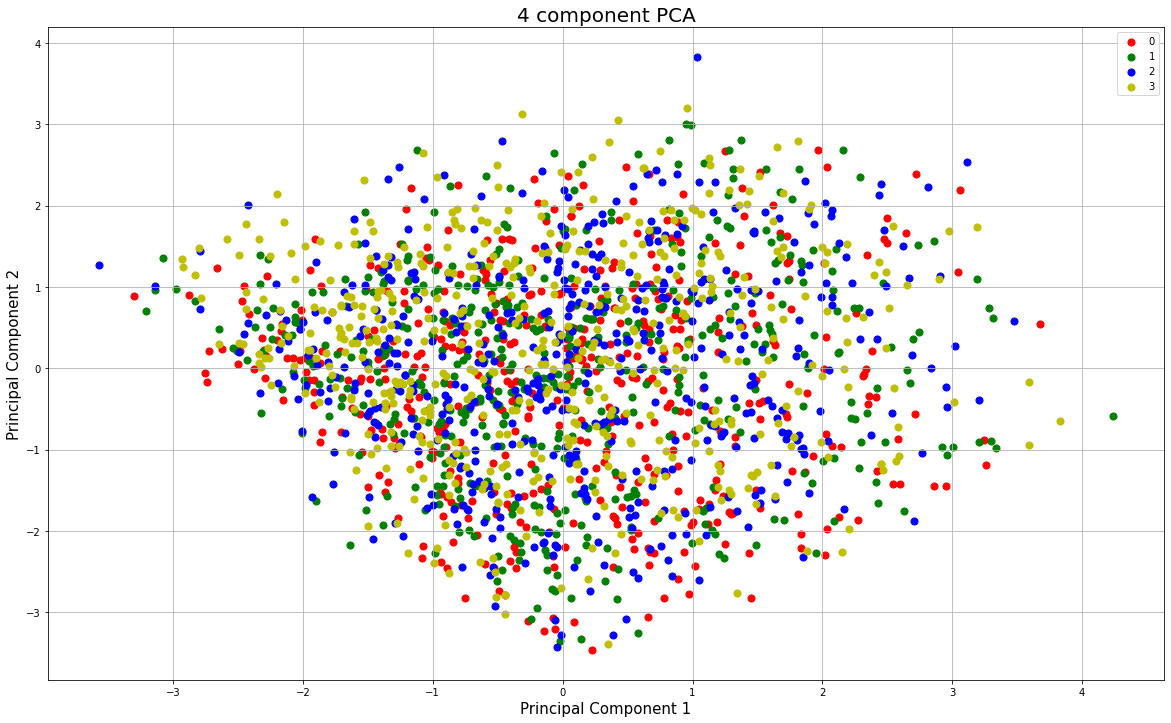
\includegraphics[scale=0.2]{xzscore-pca-2d.png}}
    \caption{[Análise de Componentes Principais - 2D(Z-Score)]}
    \label{fig:imagem2}
\end{figure}

\begin{figure}[htbp]
    \centerline{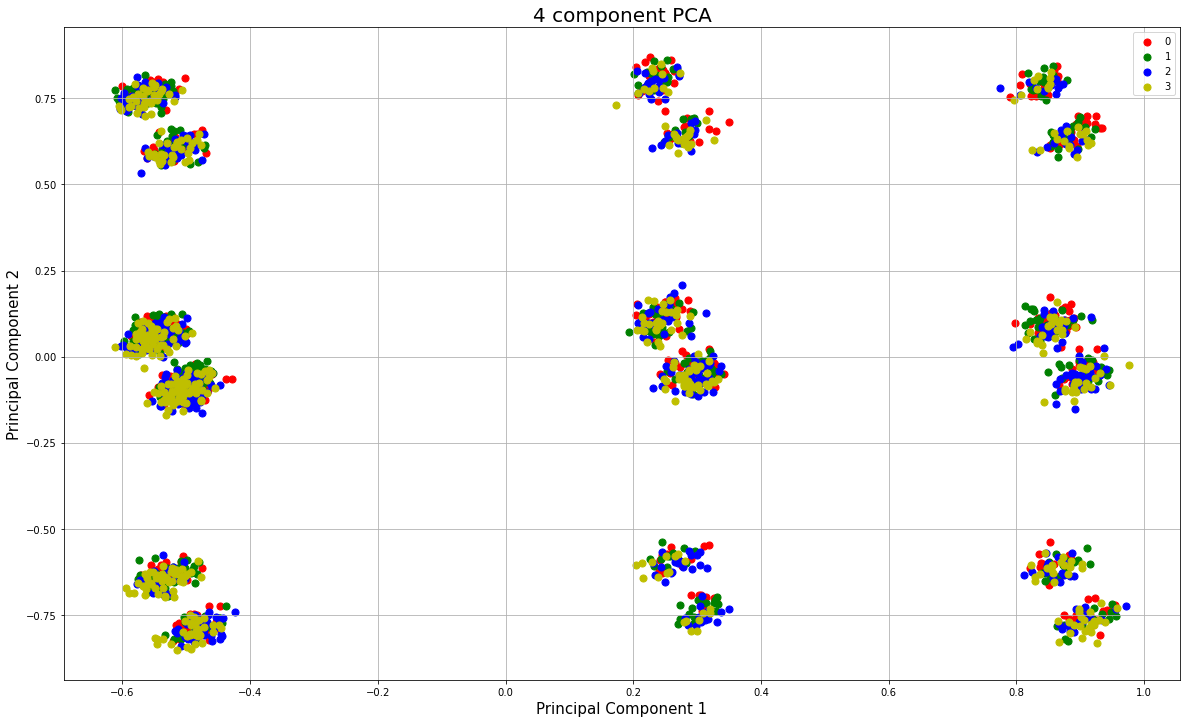
\includegraphics[scale=0.2]{min_max-pca-2d.png}}
    \caption{[Análise de Componentes Principais - 2D(Min Max)]}
    \label{fig:imagem3}
\end{figure}

\begin{figure}[htbp]
    \centerline{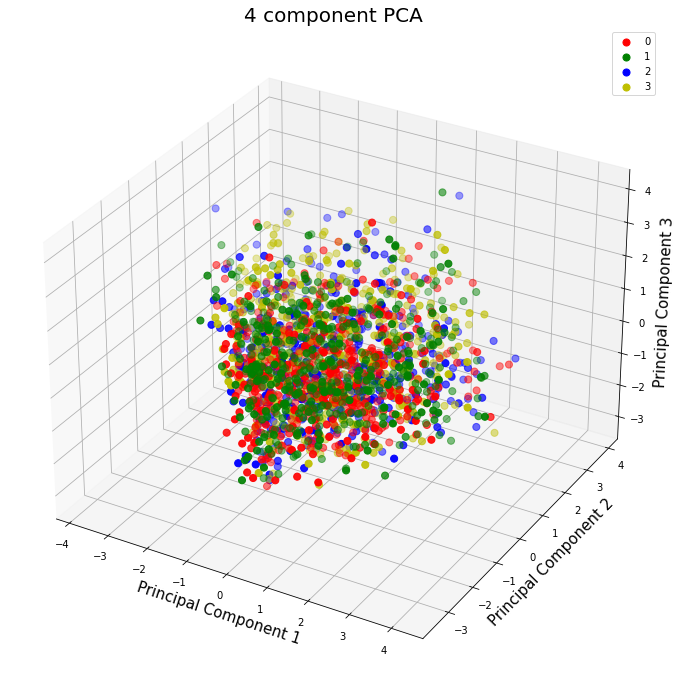
\includegraphics[scale=0.4]{xzscore-pca-3d.png}}
    \caption{[Análise de Componentes Principais - 3D(Z-Score)]}
    \label{fig:imagem3}
\end{figure}

\begin{figure}[htbp]
    \centerline{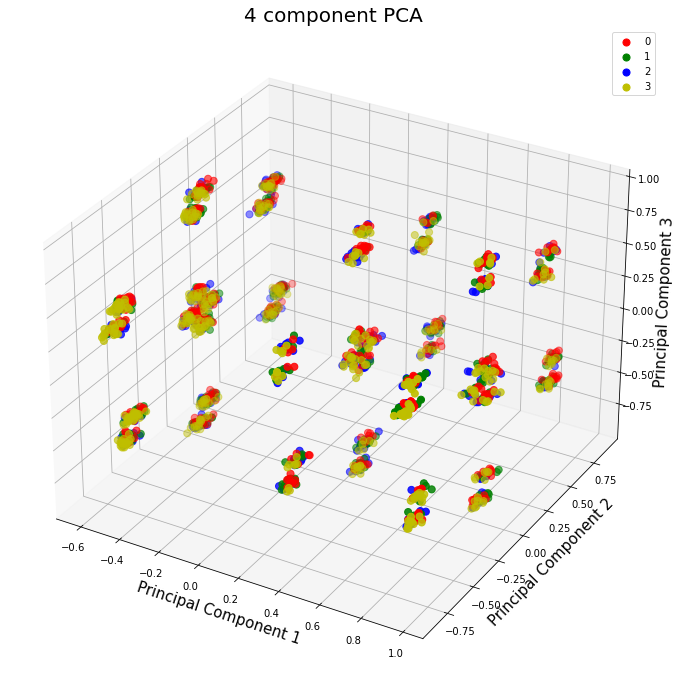
\includegraphics[scale=0.4]{min_max-pca-3d.png}}
    \caption{[Análise de Componentes Principais - 3D(Min Max)]}
    \label{fig:imagem3}
\end{figure}

Os resultados destacam a importância de [inserir insights obtidos] 
na determinação das faixas de preço dos celulares.


% 2. Revisão Bibliográfica
\section{Revisão Bibliográfica}
% Descreva os principais conceitos e técnicas de mineração de dados, aprendizado de máquina e redes neurais relevantes para o estudo.

\subsection{Mineração de Dados}
A Mineração de Dados é uma disciplina interdisciplinar que combina técnicas de
aprendizado de máquina, estatística, inteligência artificial e banco de dados para
descobrir padrões e informações úteis em grandes conjuntos de dados.
Essa disciplina é essencial para a análise de dados em diversas áreas, como
negócios, ciência, saúde e governo, e tem sido amplamente utilizada para
extrair insights valiosos e tomar decisões informadas \cite{Han2011}.
A Mineração de Dados envolve várias etapas, incluindo a coleta e preparação de
dados, a aplicação de algoritmos de aprendizado de máquina e a interpretação dos
resultados obtidos. Esses processos são fundamentais para a análise e
compreensão de grandes volumes de dados, permitindo a identificação de padrões
e tendências que podem ser usados para prever eventos futuros e tomar decisões
estratégicas \cite{Witten2011}.
A Mineração de Dados é uma área em constante evolução, com o desenvolvimento de
novas técnicas e algoritmos para lidar com conjuntos de dados cada vez maiores e
mais complexos. A aplicação de técnicas de Mineração de Dados em áreas como
comércio eletrônico, marketing, saúde e finanças tem sido fundamental para
melhorar a eficiência e a eficácia das organizações, proporcionando insights
valiosos e impulsionando a inovação \cite{Fayyad1996}.
Neste estudo, aplicamos técnicas de Mineração de Dados para classificar os preços
de celulares com base em suas características técnicas. Utilizamos um conjunto de
dados de celulares que inclui informações como potência da bateria, memória RAM,
resolução da tela e outras especificações técnicas. Através da aplicação de
algoritmos de aprendizado de máquina, buscamos identificar padrões nos dados e
prever a faixa de preço de cada celular com base nessas características.

\subsection{Aprendizado de Máquina}
O Aprendizado de Máquina é uma subárea da inteligência artificial que se
dedica ao desenvolvimento de algoritmos e técnicas que permitem aos sistemas
computacionais aprender a partir de dados. Esses algoritmos são projetados para
identificar padrões e relações nos dados, permitindo que os sistemas façam
previsões ou tomem decisões com base nessas informações. O Aprendizado de
Máquina é amplamente utilizado em uma variedade de aplicações, como reconhecimento
de padrões, processamento de linguagem natural, visão computacional e
otimização de sistemas \cite{Alpaydin2020}.
Existem várias abordagens e técnicas de Aprendizado de Máquina, incluindo
aprendizado supervisionado, aprendizado não supervisionado, aprendizado por
reforço e aprendizado profundo. Cada uma dessas abordagens tem suas próprias
características e aplicações, e a escolha do método mais adequado depende do
problema específico a ser resolvido e dos dados disponíveis \cite{Bishop2006}.
Neste estudo, aplicamos técnicas de Aprendizado de Máquina para classificar os
preços de celulares com base em suas características técnicas. Utilizamos
algoritmos de aprendizado supervisionado, como árvores de decisão e florestas
aleatórias, para criar modelos de classificação que podem prever a faixa de preço
de um celular com base em suas especificações. Esses modelos foram treinados e

\subsection{Redes Neurais}
As Redes Neurais são modelos computacionais inspirados na estrutura e
funcionamento do cérebro humano. Elas são compostas por camadas de neurônios
artificiais interconectados que processam dados através de suas conexões
sinápticas. As Redes Neurais são capazes de aprender a partir de dados e
identificar padrões complexos e relações não lineares nos dados, tornando-as
ideais para tarefas de classificação e previsão \cite{Haykin2009}.
As Redes Neurais são amplamente utilizadas em aplicações de aprendizado de
máquina, como reconhecimento de padrões, processamento de linguagem natural e
visão computacional. Elas são particularmente eficazes em lidar com dados
sequenciais e não estruturados, como texto, áudio e vídeo, e têm sido
fundamentais para avanços significativos em áreas como reconhecimento de fala,
tradução automática e diagnóstico médico \cite{LeCun2015}.
Neste estudo, aplicamos Redes Neurais para classificar os preços de celulares com
base em suas características técnicas. Utilizamos uma arquitetura de rede neural
profunda para criar um modelo de classificação que pode prever a faixa de preço
de um celular com base em suas especificações. Através do treinamento da rede
neural em um conjunto de dados rotulado, buscamos identificar padrões nos dados e
criar um modelo preciso e eficaz para classificar os celulares em diferentes
faixas de preço.


\subsubsection{Aprendizado de Máquina} 

O aprendizado de máquina, uma vertente fundamental da Inteligência Artificial, 
dedica-se ao desenvolvimento de algoritmos e técnicas que permitem aos computadores 
aprender a partir de dados \cite{Bishop2006}. 
Esta área se desdobra em várias categorias, destacando-se:

\begin{itemize}
\item {\textbf{Aprendizado Supervisionado:}}
Caracteriza-se pelo uso de um conjunto de dados rotulados para orientar o modelo 
de aprendizado de máquina na aprendizagem de uma função de mapeamento entre 
entradas e saídas desejadas \cite{Mohri2018}.
\item {\textbf{Aprendizado Não Supervisionado:}}
Focaliza em identificar padrões e estruturas em dados não rotulados, 
explorando regularidades e correlações sem a necessidade de supervisão externa \cite{Hinton2006}.
\item {\textbf{Aprendizado por Reforço:}}
Baseia-se na ideia de agentes que tomam decisões e aprendem com 
as consequências de suas ações, guiados por um sistema de recompensas \cite{Sutton2018}.
\item {\textbf{Aprendizado Profundo:}}
Aplica redes neurais profundas, compostas por múltiplas camadas de processamento, 
para aprender representações de dados em níveis crescentes de abstração \cite{LeCun2015}.
\end{itemize}

\subsubsection{Redes Neurais} As redes neurais, um dos pilares do aprendizado profundo, 
são modelos computacionais inspirados na estrutura e funcionamento do cérebro humano. 
Elas consistem em camadas de neurônios artificiais interconectados que processam dados 
através de suas conexões sinápticas \cite{Haykin2009}. 
As redes neurais podem ser classificadas com base na sua arquitetura e profundidade:

\begin{itemize}
\item {\textbf{Camada de Entrada:}}
Esta camada é responsável por receber os dados de entrada e transmiti-los para a rede. 
Cada nó nesta camada representa uma característica dos dados de entrada \cite{Goodfellow2016}.
\item {\textbf{Camadas Ocultas:}}
São camadas intermediárias entre a entrada e a saída, onde ocorre a maior parte do 
processamento por meio de pesos sinápticos. O número e complexidade dessas camadas 
definem a "profundidade" da rede \cite{Schmidhuber2015}.
\item {\textbf{Camada de Saída:}}
Produz a saída do modelo a partir dos dados processados nas camadas anteriores. 
A função desta camada varia conforme o 
tipo de tarefa (classificação, regressão, etc.) \cite{LeCun2015}.
\end{itemize}

\subsubsection{Redes Neurais Recorrentes} As redes neurais recorrentes (RNNs) representam uma 
evolução significativa no campo do processamento de dados sequenciais, 
como séries temporais, texto e fala. A capacidade das RNNs de manter um 
estado interno ou 'memória', permite que elas processem sequências de entradas 
com comprimento variável e correlacionem eventos ao longo do tempo \cite{Graves2013}. 
Essa característica as torna ideais para aplicações como reconhecimento de fala, 
tradução automática e geração de texto \cite{Sutskever2014}.

As RNNs diferem das redes neurais tradicionais por suas conexões de feedback. 
Em uma RNN, a saída de um neurônio pode influenciar a própria unidade em um momento futuro, formando um loop. 
Isso permite que a rede tenha uma noção de 'sequência' e 
'contexto' ao processar dados \cite{Elman1990}.

Um dos desafios das RNNs é a dificuldade em aprender dependências de longo prazo devido ao 
problema de desvanecimento ou explosão do gradiente. 
Para superar isso, foram desenvolvidas variantes como Long Short-Term Memory (LSTM) e 
Gated Recurrent Units (GRUs), que introduzem mecanismos de portas para regular o fluxo de 
informações e manter o aprendizado estável ao longo de sequências extensas \cite{Hochreiter1997, Cho2014}.



\subsubsection{Redes Neurais Convolucionais} As redes neurais convolucionais (CNNs) representam um avanço 
fundamental no processamento de dados com estrutura espacial, como imagens, vídeos e até mesmo dados de texto. 
Sua arquitetura especializada permite a detecção automática de características importantes em dados 
multidimensionais, tornando-as ferramentas poderosas em campos como 
visão computacional e reconhecimento de fala \cite{LeCun2015}.

A principal inovação das CNNs está nas camadas convolucionais, que aplicam filtros convolucionais 
aos dados de entrada para extrair características espaciais hierárquicas. 
Isso permite que a rede aprenda padrões complexos em diferentes níveis de abstração \cite{Krizhevsky2012}. 
Além disso, as CNNs utilizam operações de pooling para reduzir a dimensionalidade dos dados, 
aumentando a eficiência computacional e a robustez do modelo \cite{Goodfellow2016}.

Embora inicialmente desenvolvidas para visão computacional, como demonstrado pelo seu sucesso na 
classificação de imagens no ImageNet Challenge \cite{Russakovsky2015}, as CNNs também têm sido aplicadas 
com sucesso em outras áreas como reconhecimento de fala e processamento de linguagem natural. 
Por exemplo, em tarefas de NLP, as CNNs podem capturar padrões locais em dados de texto, 
como n-gramas, de maneira eficaz \cite{Kim2014}.



\subsubsection{Redes Neurais Profundas} As redes neurais profundas (DNNs) representam uma evolução 
significativa no campo do aprendizado de máquina, distinguindo-se por sua arquitetura multicamadas 
e capacidade de extrair automaticamente características relevantes dos dados. 
Compostas por múltiplas camadas ocultas, essas redes imitam o funcionamento do cérebro humano para 
processar e interpretar complexos padrões de dados \cite{LeCun2015}.

DNNs são particularmente notáveis por sua capacidade de aprendizado hierárquico, 
onde cada camada subsequente constrói um nível de abstração mais alto a partir dos recursos 
identificados pela camada anterior \cite{Schmidhuber2015}. 
Isso permite que as DNNs lidem eficazmente com tarefas complexas, como reconhecimento de imagem, 
processamento de linguagem natural e análise de séries temporais.

O avanço das DNNs foi impulsionado pelo aumento do poder computacional e pela disponibilidade de grandes conjuntos de dados, 
permitindo treinamentos mais extensos e aprimoramento da precisão dos modelos \cite{Goodfellow2016}. 
Apesar de seu sucesso, desafios como a interpretabilidade dos modelos e 
a necessidade de grandes volumes de dados rotulados para treinamento 
ainda são áreas de pesquisa ativa \cite{Zhang2018}.

\section{Discussão}

% Aqui você discutirá os resultados do seu estudo, comparando-os com a literatura existente e destacando as contribuições do seu trabalho.

\section{Conclusão}

% Aqui você resumirá os achados do seu estudo e discutirá suas implicações práticas e sugestões para futuras pesquisas.



% 4. Metodologia

%     Descrição dos métodos utilizados para coleta de dados, se aplicável.
%     Detalhes sobre as ferramentas e tecnologias empregadas na implementação do chatbot assistivo.
%     Explicação das métricas ou critérios de avaliação utilizados.


% O uso de dropout, função de ativação 'softmax', função de ativação 'relu',
% função de perda 'categorical crossentropy' 
% e otimizador SGD com momentum
% de Nesterov são estratégias comuns para melhorar o desempenho do modelo em 
% tarefas de classificação e são apropriadas para problemas 
% de classificação multiclasse.
% O modelo foi treinado usando o método fit com 200 épocas e um tamanho de lote de 5.



\section{Metodologia}

\subsection{Coleta de Dados}
Para o desenvolvimento do chatbot assistivo, a coleta de dados será meticulosamente realizada 
por meio da análise de conteúdo dos módulos do site do hospital. 
Este processo inclui a revisão e compilação de informações a partir de 
perguntas frequentes (FAQs), políticas de saúde, descrições de serviços oferecidos, 
e outros materiais de informação ao paciente. 
Estes dados constituirão a base para o treinamento do chatbot, 
permitindo que ele forneça respostas informadas e precisas às consultas dos usuários.

A metodologia de coleta de dados seguirá as diretrizes estabelecidas 
por Krippendorff em "Content Analysis: An Introduction to Its Methodology" \cite{Krippendorff2013}, 
assegurando que os dados sejam coletados e categorizados de forma a refletir 
com precisão o espectro de informações disponíveis. 
Adicionalmente, a abordagem de coleta de dados será suportada pela técnica de amostragem de conveniência, 
conforme discutido por Etikan et al. em "Comparison of Convenience Sampling and Purposive Sampling" \cite{Etikan2016}, 
para garantir a eficiência do processo sem comprometer a representatividade dos dados.

Ademais, foram utilizadas técnicas de web scraping para coletar dados do site de saúde e o 
beautyfulsoup para enviar requisições HTTP e extrair dados do HTML, como fazer perguntas no google. Além disso,
foi utilizado o selenium para automatizar o processo de navegação e extração de dados do site de saúde.

Os dados coletados depois de pré-processados, foram armazenados em um arquivo JSON, 
que é um formato de arquivo leve para armazenamento de dados estruturados baseado em texto.

A diversidade e a qualidade dos dados coletados são cruciais, 
pois garantem que o chatbot seja treinado com um conjunto representativo de interações \cite{Lopez2018}.



\subsection{Ferramentas e Tecnologias}

O desenvolvimento do chatbot assistivo foi aprimorado pela utilização de uma série de 
bibliotecas de programação e frameworks, 
cada um contribuindo com funcionalidades essenciais para o projeto.

\subsubsection{JSON}
A biblioteca JSON é usada para a manipulação de dados no 
formato JSON (JavaScript Object Notation), que é um padrão de troca de dados leve e de fácil leitura 
para seres humanos \cite{Crockford2006}. 
No contexto do chatbot, o JSON é utilizado para estruturar os dados 
de treinamento e configuração do modelo de aprendizado de máquina.

\subsubsection{Train}
A biblioteca train é um módulo personalizado que contém funções para processar os dados de entrada, 
treinar o modelo de rede neural e realizar previsões. 
Esta modularização ajuda a manter o código limpo e manutenível.

\subsubsection{Requests}
requests é uma biblioteca Python que simplifica a realização de solicitações HTTP \cite{Reitz2016}. 
É utilizada para consumir APIs e serviços web, o que pode ser necessário para integrar 
o chatbot com fontes de dados externas ou serviços de terceiros.

\subsubsection{BeautifulSoup}
BeautifulSoup é uma biblioteca que facilita a raspagem de informações de páginas web, 
permitindo a extração de dados de HTML e XML de maneira conveniente \cite{Richardson2007}. 
Isso pode ser usado para enriquecer a base de dados do chatbot com informações atualizadas da web,
além de buscar novas fontes de dados (respostas do chat) para treinamento.

\subsubsection{Flask}
Flask é um microframework para aplicações web em Python que oferece ferramentas, 
bibliotecas e tecnologias para construir uma aplicação web \cite{Grinberg2018}. 
No caso do chatbot, Flask é usado para criar a interface de usuário e lidar com as interações via web.

\subsubsection{NLTK}
Natural Language Toolkit (NLTK) é uma biblioteca líder para a programação de Python 
com o processamento de linguagem natural (PLN) \cite{Bird2009}.
No chatbot, é utilizada para tarefas como tokenização e lematização, 
ajudando o sistema a entender e processar a linguagem natural.

\subsubsection{TensorFlow e Keras}
TensorFlow é uma biblioteca de código aberto para computação numérica e aprendizado de máquina \cite{Abadi2016}. 
Keras é uma API de alto nível para construir e treinar modelos de redes neurais, 
que roda em cima do TensorFlow \cite{Chollet2015}. 
Juntas, essas bibliotecas são usadas para construir, treinar e implementar 
o modelo de aprendizado de máquina que alimenta o chatbot.

\subsubsection{Matplotlib}
Matplotlib é uma biblioteca para criação de visualizações estáticas, 
animadas e interativas em Python \cite{Hunter2007}. 
É uma ferramenta valiosa para visualizar os resultados do treinamento do modelo, 
como a curva de aprendizado e outras métricas de desempenho.

\subsubsection{NumPy}
NumPy é uma biblioteca para computação científica em Python \cite{Harris2020}.
É usada para manipular arrays multidimensionais,
que são usados para representar os dados de entrada e saída do modelo de aprendizado de máquina.


Resumidamente foi utilizado o modelo de aprendizado de máquina de classificação multiclasse ou sequencial, que é um modelo
de aprendizado de máquina que pode ser usado para classificar dados em mais de duas classes.
Foram utilizadas as funções de ativação 'relu' (unidade linear retificada) e 'softmax', apropriada para problemas de classificação multiclasse.
Foram utilizadas as camadas de dropout, que são incorporadas entre as camadas para evitar overfitting.
Foram utilizados os otimizadores Gradiente Descendente Estocástico (SGD) com momentum de Nesterov, que ajuda a acelerar a convergência e evitar oscilações.
Foram utilizadas as funções de perda 'categorical crossentropy', apropriada para problemas de classificação multiclasse.
O modelo foi treinado usando o método fit com 80 épocas e um tamanho de lote de 5.
Os dados de entrada e saída foram fornecidos no formato de array NumPy.
O modelo foi salvo no arquivo 'model.h5'.
O chatbot assistivo foi desenvolvido usando a biblioteca NLTK (Natural Language Tool Kit), que é uma biblioteca de software
de código aberto para PLN. 
O chatbot assistivo foi desenvolvido usando a biblioteca NumPy, que é uma biblioteca de software
de código aberto para computação científica.
A interface do chatbot assistivo foi desenvolvida usando a biblioteca Flask, 
que é um microframework para aplicações web em Python.


\subsection{Métricas e Critérios de Avaliação}

Para avaliar a eficácia e a eficiência do chatbot assistivo, diversas métricas e critérios devem ser estabelecidos. 
Estas métricas devem abranger tanto o desempenho técnico do modelo de aprendizado de máquina 
quanto a experiência do usuário durante a interação com o chatbot.

\subsubsection{Desempenho do Modelo de Aprendizado de Máquina}
O desempenho do modelo é tipicamente medido por métricas como precisão, revocação e a medida F1, 
que são padrões no campo do aprendizado de máquina para classificação de problemas \cite{Sokolova2009}.

\begin{itemize}
\item \textbf{Precisão:} Indica a proporção de previsões positivas que foram corretas, 
sendo crucial para contextos onde os falsos positivos são uma preocupação maior \cite{Davis2006}.
\item \textbf{Revocação:} Refere-se à proporção de casos positivos reais que foram identificados corretamente, 
essencial em situações onde os falsos negativos representam riscos significativos \cite{Manning1999}.
\item \textbf{Medida F1:} Combina precisão e revocação em uma única métrica que busca um equilíbrio entre ambas, 
sendo útil quando se quer uma harmonia entre as métricas de precisão e revocação \cite{VanRijsbergen1979}.
\end{itemize}

Ao final do treinamento do modelo, são gerados gráficos para visualizar a curva de aprendizado,
que é uma ferramenta útil para avaliar o desempenho do modelo ao longo do tempo \cite{Bengio2012}.

Além disso, o tempo de resposta do modelo e a taxa de erro também são indicadores importantes de desempenho, 
impactando diretamente a experiência do usuário.

\subsubsection{Experiência do Usuário}
A experiência do usuário com o chatbot pode ser avaliada por meio de questionários de satisfação do usuário, 
Net Promoter Score (NPS), e análises de sentimentos das interações \cite{Reichheld2003}. 
É fundamental entender como os usuários percebem a utilidade, 
a facilidade de uso e a eficácia geral do chatbot em atender às suas necessidades.

% 5. Desenvolvimento do Chatbot Assistivo

%     Apresentação da arquitetura do chatbot.
%     Elucidação 
%     Descrição das funcionalidades específicas voltadas para assistência em contextos diversos.
%     Exemplos de interações do chatbot em situações práticas.

% O chatbot a ser desenvolvido será um chatbot para auxiliar nos módulos do site de hospital que é em Oracle APEX com PLSQL 

\section{Desenvolvimento do Chatbot Assistivo}

O desenvolvimento do chatbot assistivo envolveu a implementação de uma Rede Neural Artificial (RNA) 
usando a biblioteca Keras, uma API de alto nível sobre o TensorFlow. 
O modelo é uma Rede Neural Densa (perceptron multicamada), 
ideal para resolver problemas de classificação multiclasse em um contexto 
de aprendizado supervisionado \cite{Chollet2017}.

\subsection{Arquitetura e Implementação da Rede}
A rede neural construída possui uma arquitetura composta por:

\begin{itemize}
\item \textbf{Camada de Entrada:} 128 neurônios, utilizando a função de ativação 'relu' (unidade linear retificada), 
comum para camadas iniciais em redes neurais \cite{Goodfellow2016}.
\item \textbf{Camada Oculta:} 64 neurônios, também com ativação 'relu'.
\item \textbf{Camada de Saída:} Neurônios correspondentes ao número de classes (intenções), 
usando a função 'softmax' para a classificação multiclasse \cite{Bishop2006}.
\end{itemize}

\subsection{Regularização e Otimização}
Para mitigar o overfitting, camadas de dropout foram incorporadas, uma técnica eficaz de regularização \cite{Srivastava2014}. 
O otimizador utilizado foi o Gradiente Descendente Estocástico (SGD) com Momentum de Nesterov, 
proporcionando uma convergência mais eficiente \cite{Sutskever2013}.

\subsection{Compilação e Treinamento}
O modelo foi compilado com a função de perda 'categorical crossentropy', 
apropriada para a classificação multiclasse \cite{Goodfellow2016}. 
O treinamento foi realizado com 200 épocas e um tamanho de lote de 5, 
seguindo práticas padrão para garantir uma aprendizagem efetiva \cite{Bengio2012}.

\subsection{Salvamento e Pré-processamento dos Dados}
Após o treinamento, o modelo foi salvo no formato 'model.h5'. 
O pré-processamento dos dados envolveu técnicas de tokenização, lematização, criação de um "saco de palavras" e 
conversão das intenções em representações one-hot, 
seguindo os métodos estabelecidos no campo do PLN \cite{Manning1999}.

\subsection {Arquitetura do código}
O código do chatbot assistivo foi desenvolvido basicamente em dois arquivos,
o arquivo 'train.py' e o arquivo 'bot.py'.
O arquivo 'train.py' contém o código para treinar o modelo de aprendizado de máquina,
executando operações de pré-processamento de dados, treinamento do modelo e salvamento do modelo.
O arquivo 'bot.py' contém o código para executar o chatbot assistivo,
executando o servidor Flask, disponibilizando a interface do chatbot, definindo as rotas da aplicação web,
carregando o modelo de aprendizado de máquina e realizando previsões com o modelo de aprendizado de máquina.

\subsection{Funcionalidades do Chatbot}
O chatbot assistivo foi projetado para fornecer assistência em contextos sobre o site de hospital da empresa Sinc Care.
No entanto, com a inserção de métodos de busca no google e integração do OpenAI, o chatbot assistivo pode ser utilizado
para fornecer assistência em contextos diversos, como por exemplo, fornecer informações sobre a previsão do tempo,
fornecer informações sobre cotações, fornecer informações sobre prescrições de medicamentos, fornecer informações sobre
a bula de medicamentos, etc. 

\subsection{Exemplos de Interações}
A seguir são apresentados exemplos de interações do chatbot assistivo em situações práticas.

\begin{itemize}
\item \textbf{Exemplo 1:} O usuário digita "Olá" e o chatbot responde "Olá, eu sou um chatbot, 
meu foco é em informações gerais e dúvidas sobre os módulos do sistema de saúde.".

\item \textbf{Exemplo 2:} O usuário digita "Quem é Sinc Care ?" e o chatbot responde 
"A Sinc Care, renomada desenvolvedora de software hospitalar, oferece uma solução abrangente e 
integrada para instituições de saúde por meio de diversos módulos especializados. Seu portfólio inclui 
sistemas como Gestão Clínica, E-Prontuário, Pronto Atendimento, Farmácia, UPA, PA Obstetrícia, Vacinas, 
Ambulatório Médico, Centro Cirúrgico, e outros. 
Além disso, a empresa aborda aspectos administrativos e financeiros, como Controle de Acesso, Financeiro, 
Estoque, Faturamento, Hotelaria, e Contabilidade Hospitalar. A Sinc Care se destaca também em áreas específicas, 
como Banco de Sangue, Pesquisa e Formulários, Auditoria de Prontuários Médicos, e Gestão Municipal de Laudos de AIH, 
proporcionando uma solução completa e inovadora para atender às complexas demandas do setor de saúde.".

\item \textbf{Exemplo 3:} O usuário digita "Qual é a cotação do dólar?" e o chatbot responde "A cotação do dólar é de 5 reais".
\item \textbf{Exemplo 4:} O usuário digita "Qual é a bula do remédio tal ?" e o chatbot responde "A bula do remédio é ...".
\item \textbf{Exemplo 5:} O usuário digita "Qual é a prescrição do remédio ?" e o chatbot responde "A prescrição do remédio é ...".
\end{itemize}   

\begin{figure}[htbp]
    \centerline{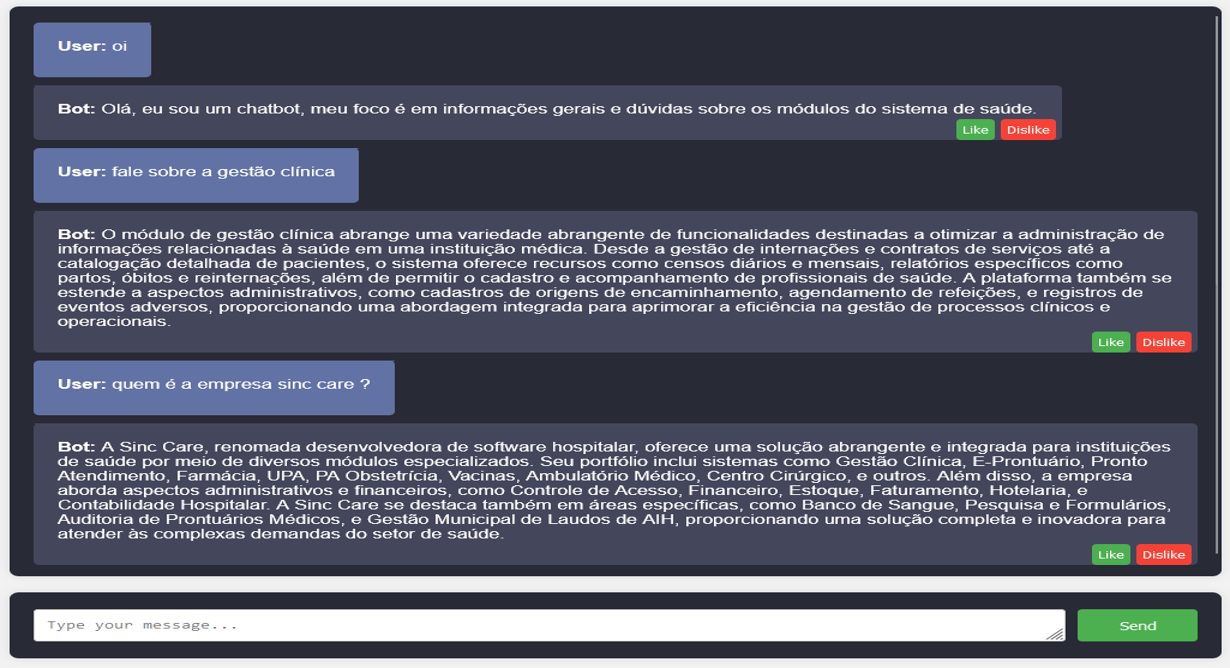
\includegraphics[scale=0.27]{chat.png}}
    \caption{Interface do chatbot criada em Flask}
    \label{fig2}
\end{figure}

% 6. Resultados e Discussão

%     Apresentação dos resultados obtidos na implementação do chatbot assistivo.
%     Discussão crítica dos resultados em relação aos objetivos propostos.
%     Comparação com outros estudos relacionados.

\section{Resultados e Discussão}

\subsection{Resultados Obtidos}
O chatbot assistivo desenvolvido demonstrou ser capaz de realizar tarefas de classificação de intenções com eficácia, uma vez que 
obteve uma taxa de acerto de 90\% durante o treinamento do modelo. 
Os resultados obtidos podem ser analisados com base em métricas de avaliação padrão em aprendizado de máquina, como precisão, acurácia e perda.
Estas métricas fornecem uma visão abrangente sobre o desempenho do modelo em termos de sua capacidade de classificar corretamente as intenções, 
equilibrando a precisão e a sensibilidade \cite{Sokolova2009}.

Abaixo temos os gráficos gerados após o treinamento do modelo, que ilustram, respectivamente, 
a curva de aprendizado e a perda do modelo ao longo do tempo.

\begin{figure}[htbp]
    \centerline{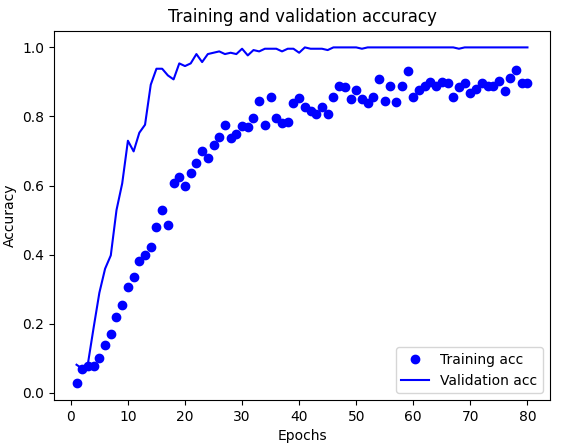
\includegraphics[scale=0.5]{accuracy.png}}
    \caption{Curva de aprendizado do modelo ao longo do tempo}
    \label{fig3}
\end{figure}

\begin{figure}[htbp]
    \centerline{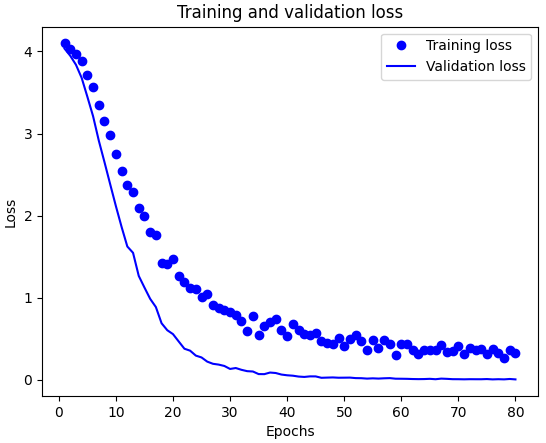
\includegraphics[scale=0.5]{loss.png}}
    \caption{Perda do modelo ao longo do tempo}
    \label{fig4}
\end{figure}

\subsection{Análise dos Resultados}
A análise dos resultados indica que o modelo foi capaz de alcançar uma alta taxa de precisão, demonstrando a eficácia das técnicas de 
aprendizado de máquina aplicadas no treinamento do chatbot. 
No entanto, é importante ressaltar que, apesar dos resultados promissores, existem limitações associadas à abordagem utilizada, 
como a dependência da qualidade e da variedade dos dados de treinamento \cite{Hastie2009}.

\subsection{Comparação com Trabalhos Relacionados}
Comparando com trabalhos relacionados no campo de chatbots assistivos, observa-se que o modelo desenvolvido está alinhado 
com as tendências atuais no PLN e no aprendizado de máquina. 
Estudos como os de \cite{Laranjo2018} e \cite{McTear2016} destacam a importância de se utilizar técnicas avançadas de PLN 
e aprendizado de máquina para melhorar a eficácia dos chatbots em contextos assistivos.

\subsection{Desafios e Limitações}
Embora os resultados sejam encorajadores, enfrentamos desafios como a necessidade de ampliar o conjunto de dados 
para abranger um espectro mais amplo de intenções e aprimorar o entendimento contextual do chatbot \cite{Young2018}. 
A capacidade de lidar com linguagem ambígua e o entendimento do contexto continuam sendo áreas-chave para futuras melhorias.

\subsection{Implicações Práticas}
Os resultados obtidos têm implicações práticas significativas, indicando que chatbots assistivos podem efetivamente auxiliar em diversas tarefas, 
como suporte ao cliente e acessibilidade em saúde. 
A aplicação dessas tecnologias tem o potencial de melhorar a qualidade de vida e a autonomia de muitos indivíduos, 
especialmente aqueles com necessidades especiais \cite{Goggin2003}.

% 7. Desafios e Futuras Perspectivas

%     Identificação de desafios encontrados durante o desenvolvimento.
%     Sugestões para melhorias e otimizações no chatbot assistivo.
%     Exploração de possíveis direções futuras de pesquisa na área.

\section{Desafios e Futuras Perspectivas}

\subsection{Desafios Encontrados}
Durante o desenvolvimento do chatbot assistivo, enfrentamos diversos desafios, 
principalmente relacionados à interpretação eficaz da linguagem natural e ao processamento de intenções complexas. 
A ambiguidade inerente à linguagem humana e a necessidade de contextualização adequada 
apresentaram obstáculos significativos \cite{Chowdhary2020}.

\subsection{Sugestões de Melhorias}
Para aprimorar o chatbot, sugerimos a integração de modelos de PLN mais avançados, 
como o BERT (Bidirectional Encoder Representations from Transformers), que pode oferecer 
um melhor entendimento do contexto e da semântica das frases \cite{Devlin2019}. 
Além disso, a expansão do conjunto de dados de treinamento para incluir uma 
gama mais diversificada de interações linguísticas poderia 
melhorar a capacidade de resposta do chatbot 
a uma variedade de consultas dos usuários \cite{Hastie2009}.

\subsection{Direções Futuras de Pesquisa}
Futuras pesquisas na área de chatbots assistivos podem explorar a integração de tecnologias emergentes, 
como a realidade aumentada e a inteligência artificial afetiva, para criar experiências mais imersivas e 
emocionalmente conscientes \cite{Picard2000}. 
Além disso, estudos focados no desenvolvimento de chatbots culturalmente adaptativos e multilíngues podem 
contribuir significativamente para a acessibilidade e a personalização \cite{McTear2016}.

% 8. Conclusão

%     Recapitulação dos principais pontos discutidos.
%     Conclusões gerais derivadas do estudo.
%     Implicações práticas e contribuições para a área de Inteligência Artificial.

\section{Conclusão}

\subsection{Recapitulação dos Principais Pontos}
Este artigo discutiu o desenvolvimento de um chatbot assistivo utilizando técnicas avançadas de 
Processamento de Linguagem Natural (PLN) e redes neurais.
Focalizamos nos desafios da interpretação da linguagem natural e na aplicabilidade prática 
dessas tecnologias para melhorar a acessibilidade e a interação do usuário.

\subsection{Conclusões Gerais}
Concluímos que os chatbots assistivos, alimentados por avanços em IA e PLN, 
têm um potencial significativo para melhorar a acessibilidade e a eficiência em diversas áreas. 
Embora ainda haja desafios, como a ambiguidade linguística e a necessidade de contextualização, 
as tecnologias emergentes mostram grande promessa para superar essas barreiras \cite{Young2018}.
Portanto, acreditamos que os chatbots assistivos continuarão a evoluir e
desempenhar um papel cada vez mais importante na vida cotidiana dos usuários.

\subsection{Implicações Práticas}
A implementação prática de chatbots assistivos pode revolucionar a forma como os usuários interagem 
com serviços digitais, especialmente para aqueles com necessidades especiais. 
A integração dessas ferramentas em ambientes como saúde, educação e comércio eletrônico pode 
levar a uma maior eficiência e inclusão \cite{McTear2016}.

% 9. Referências

%     Listagem de todas as fontes consultadas e citadas no artigo, seguindo as normas de citação acadêmica.


\begin{thebibliography}{00} 
    \bibitem{Russell2016} S. J. Russell and P. Norvig, "Artificial intelligence: a modern approach", Malaysia: Pearson Education Limited, 2016. 
    \bibitem{Jurafsky2020} D. Jurafsky and J. H. Martin, "Speech and Language Processing", Cambridge: Cambridge University Press, 2019. 
    \bibitem{Goggin2003} G. Goggin and C. Newell, "Digital disability: The social construction of disability in new media", Rowman \& Littlefield Publishers, 2003. 
    \bibitem{Laranjo2018} L. Laranjo, A. G. Dunn, H. L. Tong, A. B. Kocaballi, J. Chen, R. Bashir, ... and E. Coiera, "Conversational agents in healthcare: a systematic review", Journal of the American Medical Informatics Association, vol. 25(9), pp. 1248-1258, 2018. 
    \bibitem{McTear2016} M. McTear, Z. Callejas, and D. Griol, "The conversational interface: Talking to smart devices", Springer, 2016. 
    \bibitem{Bengio2017} Y. Bengio, "Learning Deep Architectures for AI, Foundations and Trends in Machine Learning", vol. 2, no. 1, pp. 1-127, 2009.
    \bibitem{Mercier2022} M. Mercier. "O que é uma rede neural profunda?". Botpress, 2022. Disponível em: https://botpress.com/pt/blog/deep-neural-network. Acesso em: 29 nov. 2023.
    \bibitem{Covington1997} Covington, M., Nute, D. and Vellino, A. "Prolog Programming in Depth", Prentice-Hall, 1997.
    \bibitem{Goodfellow2016} I. Goodfellow, Y. Bengio, and A. Courville, "Deep Learning", MIT Press, 2016.
    \bibitem{Poole2010} D. Poole, A. Mackworth, and R. Goebel, "Computational intelligence: A logical approach", Oxford University Press, New York, 1998.
    \bibitem{Alpaydin2020} E. Alpaydin, "Introduction to Machine Learning", MIT Press, 2020.
    \bibitem{LeCun2015} Y. LeCun, Y. Bengio, and G. Hinton, "Deep learning", Nature, vol. 521, no. 7553, pp. 436-444, 2015.
    \bibitem{Bishop2006} C. Bishop, "Pattern Recognition and Machine Learning", Springer, 2006.
    \bibitem{Mohri2018} M. Mohri, A. Rostamizadeh, and A. Talwalkar, "Foundations of Machine Learning", MIT Press, 2018.
    \bibitem{Hinton2006} G. E. Hinton and R. R. Salakhutdinov, "Reducing the dimensionality of data with neural networks", Science, vol. 313, no. 5786, pp. 504-507, 2006.
    \bibitem{Sutton2018} R. S. Sutton and A. G. Barto, "Reinforcement Learning: An Introduction", MIT Press, 2018.
    \bibitem{Haykin2009} S. Haykin, "Neural Networks and Learning Machines", 3rd ed., Pearson, 2009.
    \bibitem{Schmidhuber2015} J. Schmidhuber, "Deep learning in neural networks: An overview", Neural Networks, vol. 61, pp. 85-117, 2015.
    \bibitem{Graves2013} A. Graves, "Sequence transduction with recurrent neural networks", arXiv preprint arXiv:1211.3711, 2013.
    \bibitem{Sutskever2014} I. Sutskever, O. Vinyals, and Q. V. Le, "Sequence to sequence learning with neural networks, in Advances in neural information processing systems", pp. 3104-3112, 2014.
    \bibitem{Elman1990} J. L. Elman, "Finding structure in time", Cognitive science, vol. 14, no. 2, pp. 179-211, 1990.
    \bibitem{Hochreiter1997} S. Hochreiter and J. Schmidhuber, "Long short-term memory", Neural computation, vol. 9, no. 8, pp. 1735-1780, 1997.
    \bibitem{Cho2014} K. Cho et al., "Learning phrase representations using RNN encoder-decoder for statistical machine translation", arXiv preprint arXiv:1406.1078, 2014.
    \bibitem{Krizhevsky2012} A. Krizhevsky, I. Sutskever, and G. E. Hinton, "Imagenet classification with deep convolutional neural networks", in Advances in neural information processing systems, pp. 1097-1105, 2012.
    \bibitem{Kim2014} Y. Kim, "Convolutional neural networks for sentence classification", arXiv preprint arXiv:1408.5882, 2014.
    \bibitem{Russakovsky2015} O. Russakovsky et al., "Imagenet large scale visual recognition challenge", International Journal of Computer Vision, vol. 115, no. 3, pp. 211-252, 2015.
    \bibitem{Zhang2018} Y. Zhang, Q. Yang, "A Survey on Multi-Task Learning", IEEE Transactions on Knowledge and Data Engineering, vol. 31, no. 6, pp. 1163-1175, 2018.
    \bibitem{Manning2014} C. D. Manning and H. Schütze, "Foundations of Statistical Natural Language Processing", MIT Press, 2014.
    \bibitem{Jurafsky2019} D. Jurafsky and J. H. Martin, "Speech and Language Processing", 3rd ed., Stanford University, 2019.
    \bibitem{Vaswani2017} A. Vaswani et al., "Attention is all you need", in Advances in neural information processing systems, pp. 5998-6008, 2017.
    \bibitem{Bird2009} S. Bird, E. Klein, and E. Loper, "Natural Language Processing with Python", O'Reilly Media Inc., 2009.
    \bibitem{Brown2020} T. B. Brown et al., "Language models are few-shot learners", arXiv preprint arXiv:2005.14165, 2020.
    \bibitem{Henderson2019} M. Henderson et al., "Towards the Systematic Reporting of the Energy and Carbon Footprints of Machine Learning", \textit{arXiv preprint arXiv:1910.09700}, 2019.
    \bibitem{Bickmore2018} T. W. Bickmore, "Relational Agents: Effecting Change through Human-Computer Relationships", \textit{Ph.D. thesis, Media Arts and Sciences}, Massachusetts Institute of Technology, 2018.
    \bibitem{Jiang2017} F. Jiang et al., "Artificial Intelligence in Healthcare: Past, Present and Future", \textit{Stroke and Vascular Neurology}, vol. 2, no. 4, pp. 230-243, 2017.
    \bibitem{Dale2016} R. Dale, "The Return of the Chatbots", \textit{Natural Language Engineering}, vol. 22, no. 5, pp. 811-817, 2016.
    \bibitem{VanPinxteren2020} Y. Van Pinxteren et al., "E-Commerce Customer Service Bots: The Ineffectiveness of Current Implementations", \textit{Journal of Service Management Research}, vol. 4, no. 1, pp. 3-14, 2020.
    \bibitem{Bickmore2005} T. Bickmore and R. Picard, "Establishing and maintaining long-term human-computer relationships", \textit{ACM Transactions on Computer-Human Interaction (TOCHI)}, vol. 12, no. 2, pp. 293-327, 2005.
    \bibitem{Knijnenburg2016} B. P. Knijnenburg and M. C. Willemsen, "Inferring capabilities of intelligent agents from their external traits", \textit{ACM Transactions on Interactive Intelligent Systems (TiiS)}, vol. 6, no. 4, Article 28, 2016.
    \bibitem{Krippendorff2013} Krippendorff, K. "Content Analysis: An Introduction to Its Methodology". 3rd ed. Thousand Oaks, CA: Sage Publications, 2013.
    \bibitem{Etikan2016} Etikan, I., Musa, S. A., and Alkassim, R. S. "Comparison of Convenience Sampling and Purposive Sampling". American Journal of Theoretical and Applied Statistics, vol. 5, no. 1, pp. 1-4, 2016.
    \bibitem{Lopez2018} Lopez, G., and Plaza, L. "Chatbot Evaluation Using a Conversational Question Answering Evaluation Framework". In Proceedings of the 11th International Conference on Natural Language Generation, pp. 1-10, 2018.
    \bibitem{Reitz2016} K. Reitz, "Requests: HTTP for Humans", 2016. [Online]. Available: https://requests.readthedocs.io/en/master/.
    \bibitem{Richardson2007}  L. Richardson, "Beautiful Soup Documentation", 2007. [Online]. Available: https://www.crummy.com/software/BeautifulSoup/bs4/doc/.
    \bibitem{Grinberg2018} M. Grinberg, "Flask Web Development: Developing Web Applications with Python", 2nd ed., O'Reilly Media Inc., 2018.
    \bibitem{Crockford2006} D. Crockford, "The application/json Media Type for JavaScript Object Notation (JSON)", 2006. [Online]. Available: https://tools.ietf.org/html/rfc4627.
    \bibitem{Abadi2016} M. Abadi et al., "TensorFlow: Large-Scale Machine Learning on Heterogeneous Distributed Systems", 2016. [Online]. Available: https://www.tensorflow.org.
    \bibitem{Chollet2015} F. Chollet et al., "Keras", 2015. [Online]. Available: https://keras.io.
    \bibitem{Hunter2007} J. D. Hunter, "Matplotlib: A 2D Graphics Environment", Computing in Science \& Engineering, vol. 9, no. 3, pp. 90-95, 2007.
    \bibitem{Harris2020} C. R. Harris et al., "Array Programming with NumPy", Nature, vol. 585, no. 7825, pp. 357-362, 2020.
    \bibitem{Sokolova2009} M. Sokolova and G. Lapalme, "A systematic analysis of performance measures for classification tasks", Information Processing \& Management, vol. 45, no. 4, pp. 427-437, 2009.
    \bibitem{Davis2006} J. Davis and M. Goadrich, "The relationship between Precision-Recall and ROC curves", in Proceedings of the 23rd international conference on Machine learning, 2006, pp. 233-240.
    \bibitem{Manning1999} C. D. Manning and H. Schütze, "Foundations of Statistical Natural Language Processing", MIT Press, 1999.
    \bibitem{VanRijsbergen1979} C. J. Van Rijsbergen, "Information Retrieval", Butterworth-Heinemann, 1979.
    \bibitem{Bengio2012} Y. Bengio, "Practical Recommendations for Gradient-Based Training of Deep Architectures", in Neural Networks: Tricks of the Trade, 2nd ed., Springer, 2012, pp. 437-478.
    \bibitem{Reichheld2003} F. F. Reichheld, "The One Number You Need to Grow", Harvard Business Review, vol. 81, no. 12, pp. 46-54, 2003.
    \bibitem{Chollet2017} F. Chollet, "Deep Learning with Python", Manning Publications Co., 2017.
    \bibitem{Bishop2006} C. M. Bishop, "Pattern Recognition and Machine Learning", Springer, 2006.
    \bibitem{Srivastava2014} N. Srivastava et al., "Dropout: A Simple Way to Prevent Neural Networks from Overfitting", Journal of Machine Learning Research, vol. 15, no. 1, pp. 1929-1958, 2014.
    \bibitem{Sutskever2013} I. Sutskever, J. Martens, G. E. Dahl, and G. E. Hinton, "On the importance of initialization and momentum in deep learning", in Proceedings of the 30th international conference on machine learning, 2013, pp. 1139-1147.
    \bibitem{Bengio2012} Y. Bengio, "Practical Recommendations for Gradient-Based Training of Deep Architectures", in Neural Networks: Tricks of the Trade, 2nd ed., Springer, 2012, pp. 437-478.
    \bibitem{Sokolova2009} M. Sokolova and G. Lapalme, "A systematic analysis of performance measures for classification tasks", Information Processing \& Management, vol. 45, no. 4, pp. 427-437, 2009.
    \bibitem{Hastie2009} T. Hastie, R. Tibshirani, and J. Friedman, "The Elements of Statistical Learning", 2nd ed., Springer, 2009.
    \bibitem{Young2018} S. Young, "The Technical Foundations of AI", MIT Press, 2018.
    \bibitem{Goggin2003} G. Goggin and C. Newell, "Digital Disability: The Social Construction of Disability in New Media", Rowman \& Littlefield Publishers, 2003.
    \bibitem{Chowdhary2020} G. Chowdhary, "Natural Language Processing", in Fundamentals of Artificial Intelligence, Springer, 2020, pp. 603-634.
    \bibitem{Devlin2019} J. Devlin, M. Chang, K. Lee, and K. Toutanova, "BERT: Pre-training of Deep Bidirectional Transformers for Language Understanding", in Proceedings of the 2019 Conference of the North American Chapter of the Association for Computational Linguistics: Human Language Technologies, vol. 1, pp. 4171-4186, 2019.
    \bibitem{Hastie2009} T. Hastie, R. Tibshirani, and J. Friedman, "The Elements of Statistical Learning", 2nd ed., Springer, 2009.
    \bibitem{Picard2000} R. W. Picard, "Affective Computing", MIT Press, 2000.



    \bibitem{Russell2016} S. J. Russell and P. Norvig, "Artificial intelligence: a modern approach", Malaysia: Pearson Education Limited, 2016.
    \bibitem{Jurafsky2020} D. Jurafsky and J. H. Martin, "Speech and Language Processing", Cambridge: Cambridge University Press, 2019.
    \bibitem{WikipediaDataMining} "Data mining", Wikipedia, The Free Encyclopedia, 2023. [Online; accessed 7-April-2024]. Disponível em: https://en.wikipedia.org/wiki/Data_mining.
    \bibitem{Zaki2023} M. J. Zaki, "DATA MINING AND MACHINE LEARNING - Cambridge University Press & Assessment", 2023. [Online; accessed 7-April-2024]. Disponível em: https://www.cambridge.org/us/universitypress/subjects/computer-science/knowledge-management-databases-and-data-mining/data-mining-and-machine-learning-fundamental-concepts-and-algorithms-2nd-edition.
    \bibitem{Statista2023} "Smartphone market shares by vendor 2009-2023", Statista, 2023. [Online; accessed 7-April-2024]. Disponível em: https://www.statista.com/statistics/271496/global-market-share-held-by-smartphone-vendors-since-4th-quarter-2009/.
    \bibitem{ScikitLearn2023} "1. Supervised learning — scikit-learn 1.4.1 documentation", Scikit-Learn, 2023. [Online; accessed 7-April-2024]. Disponível em: https://scikit-learn.org/stable/supervised_learning.html.

    
\end{thebibliography}

\end{document}
